\chapter{Methodik}

Nachfolgdend wird die vollständige Vorgehensweise der Versuchsdurchführung erklärt.
Dazu ist es notwendig eine Methodik zu definieren.

In der Browserforensik ist eine definierte Methodik notwendig, um die Komplexität moderner Browser zu bewältigen. Sie bildet bildet eine wissenschaftliche Basis für den durchgeführten Versuch sowie einen Leitfaden für Ermittler bei zukünftigen Untersuchungen. \cite{Aggarwal.2010, Izzati.2022, Horsman.2019}	
Ein oft verwendetes Vorgehensmodell in der Computer Forensik ist das "Generic Model Computer Forensics Investigations", kurz GCFIM. \cite{Yusoff.2011}
Ähnlich zum "abschnittsbasierter Verlauf einer forensischen Untersuchung" des Bundesamt für Sicherheit in der Informationstechnik ist es in Phasen mit definierten Abläufen gegliedert.
% https://www.bsi.bund.de/SharedDocs/Downloads/DE/BSI/Cyber-Sicherheit/Themen/Leitfaden_IT-Forensik.pdf?__blob=publicationFile&v=2

Izzati et al. haben diese Phasen auf Browserforensik abgebildet: \cite{Izzati.2022}
\begin{itemize}
	\item Vorbereitung: Versuchsplanung und Konfiguration der Versuchsumgebung.
	\item Datensammlung: Speicherabbilder identifizieren und während des Browsing Szenarios erstellen. 
	\item Datenanalyse: Suche nach Browsing Artefakten in gesammelten Daten.
	\item Dokumentation: Vorgehensweise und gefundene Artefakte dokumentieren.
\end{itemize}

Die Dokumentationsphase entspricht in dieser Arbeit Kapitel "Vergleich der Browser" (TODO!). Die Methodik der anderen Phasen wird nachfolgend beschrieben.

\section{Vorbereitung}

In der Vorbereitungsphase wird der durchgeführte Versuch geplant sowie die Versuchsumgebung konfiguriert. \cite{Izzati.2022} Versuchsplanung zählt die Auswahl von Browsern und Tools sowie die Definition eines durchzuführenden Browsing-Szenarios. Die Konfiguration der Versuchsumgebung umfasst die Installation und Konfiguration der notwendigen Software und Hardware.

\subsection{Browserauswahl}

Für diese Arbeit dazu entschieden: zwei weit verbreitete Brower verwenden + zwei Browser mit verstärkem Schutz der Privatsphäre.

Laut Statistik "Global market share held by leading internet browsers from January 2012 to May 2023" (Stand 23. Mai 2023) von Statista ist Chrome mit 62,82\% der meistgenutzte Browser weltweit.
Danach folgen Safari (20,86\%), Edge (5,28\%) und Firefox (2,77\%). 
\begin{figure}[h!]
	\resizebox{\linewidth}{!}{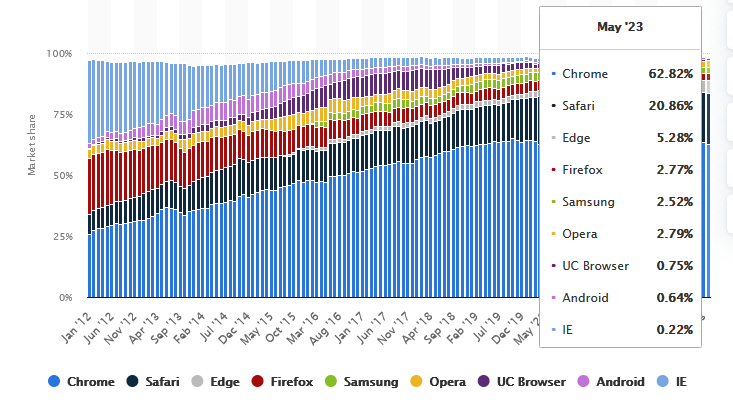
\includegraphics{bilder/browser-marketshare.png}}
%	\label{...}
	\caption{Tabelle mit wiederherstellbaren Dateien: Logfile 1 vs. Logfile 2}
\end{figure}

Problem: Safari hauptsächlich auf Mac OS genutzt, für Windows nur Safari 5.1.7 oder ältere Versionen.
Weiteres Problem: In Literatur zwar oft Internet Explorer (TODO: Quellen) untersucht, den Nachfolger Edge wurde bisher jedoch kaum in Literatur betrachtet.
	-> Nur 3 von 23 untersuchten Papern nahmen Edge mit in die Lister der analysierten Browser auf: \cite{Fayyad.2021, Horsman.2019, Gabet.2018}
	-> Ziel der Arbeit: keine neuen wissenschaftlichen Erkenntnisse.

Deshalb: wird neben Chrome noch Firefox als zweiter "regulärer" Browser aufgenommen:
Sowohl Firefox als auch Chrome werden in 15 von 23 untersuchten Papern analysiert: \cite{Aggarwal.2010, Oh.2011, Said.2011, Ohana.2013, Satvat.2014, Montasari.2015, Nalawade.2016, Rochmadi.2017, Gabet.2018, Md.2018, Muir.2019, Horsman.2019, Mahlous.2020, Fayyad.2021, Izzati.2022}

Weiterhin werden zwei Browser mit verstärkem Schutz der Privatsphäre ausgewählt.
Um die Browser mit den regulären Browsern vergleichen zu können, werden Browser gewählt, die auf den regulären Browsern basieren.
Basierend auf Chromium wird der Browser "Brave" gewählt.
Für Firefox wird der Tor-Browser gewählt, eine modifizierte Version von Firefox.

\subsubsection*{Firefox}

Der Browser Mozilla Firefox, kurz Firefox, ist ein open-source Webbrowser der gemeinnützigen Organisation Mozilla. 
Seit seiner Einführung im Jahr 2004 hat sich Firefox als beliebter Webbrowser etabliert. 

Mozilla bewirbt den Firefox Browser mit seinem Fokus Privatsphäre und Sicherheit.
Im Jahr 2009 führte Firefox den "privaten Modus" ein, der es Benutzern ermöglichte, das Surfen im Internet ohne Speicherung von Verlaufsdaten und Cookies zu genießen.
Abbildung X und Y (TODO!) zeigen, die Aktivierung des privaten Modus über das Menü in der rechten oberen Fensterecke. Der private Modus öffnet sich anschließend in einem neuen Firefox-Fenster

\begin{figure}[h!]
	\resizebox{\linewidth}{!}{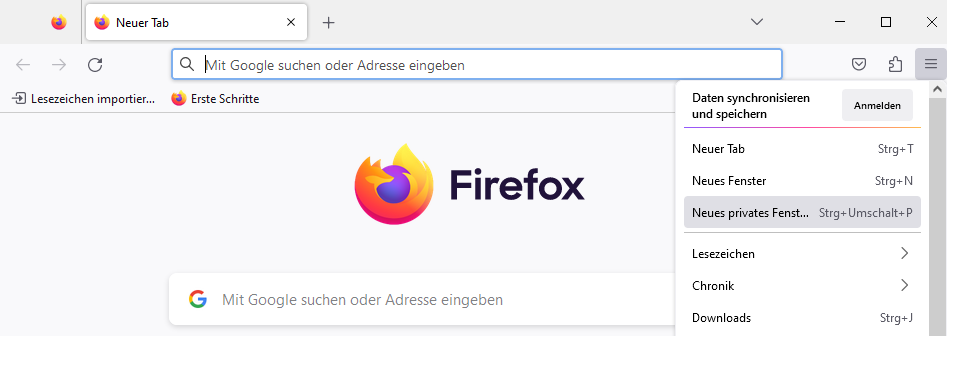
\includegraphics{bilder/firefox-private-mode.png}}
%	\label{...}
	\caption{Private Mode Firefox 1}
\end{figure}

\begin{figure}[h!]
	\resizebox{\linewidth}{!}{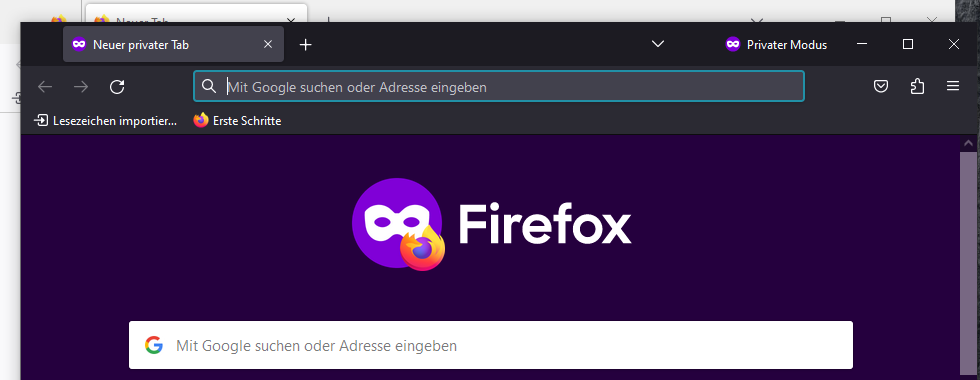
\includegraphics{bilder/firefox-private-mode2.png}}
%	\label{...}
	\caption{Private Mode Firefox 2}
\end{figure}

- Mozilla garantiert über den privaten Modus, dass Surfaktivitäten vor anderen Personen verborgen werden, die Firefox am selben Computer wie Sie verwenden. 
- Dazu zählt laut Mozilla: Passwörter, Chronik und Cookies gespeichert werden.
Dies Entspricht dem Schutz gegenüber des "Lokalen Angreifers", wie er in Kapitel X (TODO!) definiert ist.
- Es wird ausdrücklich darauf hingewiesen, dass die besuchten Webseiten und Ihr Internetanbieter (ISP)  weiterhin anhand Ihrer IP-Adresse Informationen über die von Ihnen besuchten Seiten sammeln, selbst wenn Sie nicht angemeldet sind. 
% https://www.mozilla.org/de/firefox/
% https://www.mozilla.org/de/about/history/

Somit ist der private Modus von Firefox laut Mozilla vor dem lokalen Angreifer geschützt, jedoch nicht vor dem Webangreifer.

Für diesen Versuch: Firefox Version 112.0.2 (64 Bit)

\subsubsection*{Tor}

Der Tor Browser, früher Tor Browser Bundle, ist ein auf Firefox basierender Webbrowser, der das Tor-Netzwerk nutzt.
- wird von der gemeinnützigen Organisation "The Tor Project" entwickelt
- Das Tor-Netzwerk ist ein Netzwerk virtueller Tunnel, der den Datenverkehr über drei zufällige Server ("Relays") im Tor-Netzwerk leitet, bevor er über den letzten Server (Exit-Relay) ins öffentliche Internet gelangt.
- Jedes Relay kennt nur den vorherigen und den nächsten Schritt des Datenverkehrs, aber nicht den gesamten Pfad oder die Quelle der Verbindung.
- Dadurch soll Privatsphäre und Sicherheit im Internet geschützt und verbessert werden.
- Das Tor-Netzwerk wird von einer dezentralen Community von Freiwilligen betrieben und verwaltet
- Der Tor Browser ermöglicht es Benutzern, Domains mit .onion als Top-Level-Domain zu besuchen. Die Domainnamen werden kryptografisch generiert und lassen nicht auf den Webseitennamen schließen. 

Über Tor-Browser mit Tor-Netzwerk verbinden:
\begin{figure}[h!]
	\centerline{\resizebox{\linewidth}{!}{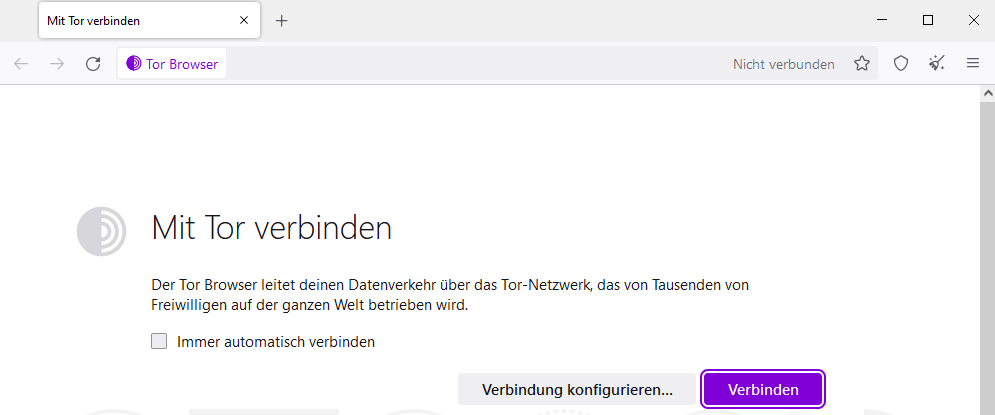
\includegraphics{bilder/tor-connect1.png}}}
%	\label{...}
	\caption{Tabelle mit wiederherstellbaren Dateien: Logfile 1 vs. Logfile 2}
\end{figure}
\begin{figure}[h!]
	\centerline{\resizebox{\linewidth}{!}{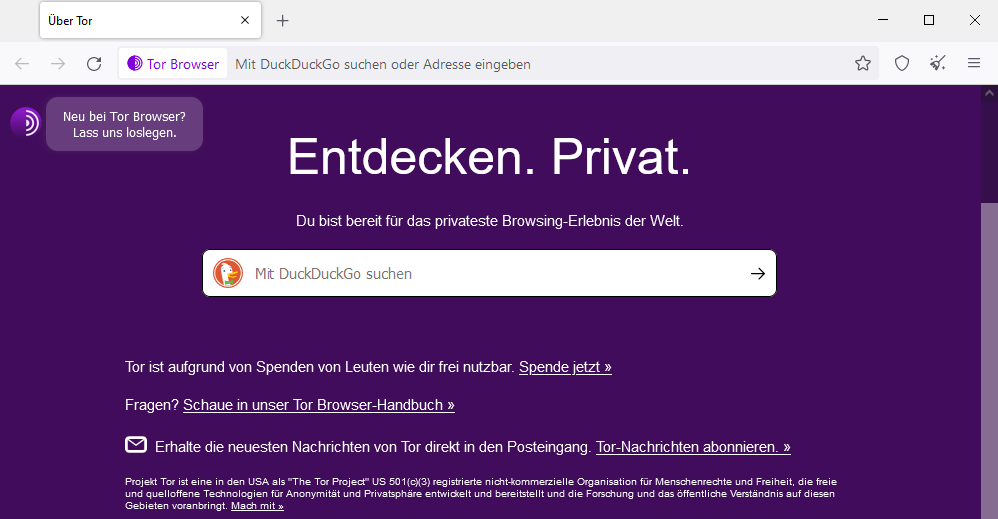
\includegraphics{bilder/tor-connect2.png}}}
%	\label{...}
	\caption{Tabelle mit wiederherstellbaren Dateien: Logfile 1 vs. Logfile 2}
\end{figure}

Der Tor Browser wirbt im Gegensatz zu Firefox mit folgendem Schutzmaßnahmen gegen Webangreifer:
- Internetdienstanbieter können Internetaktivitäten aufgrund Natur des Tor-Netzwerks nicht verfolgen 
- Die Betreiber der besuchten Websites sehen eine Verbindung vom Tor-Netzwerk anstelle der echten IP-Adresse des Rechners
- Kein "fingerprinting” = Nutzer anhand Browserkonfiguration identifizieren.

Der Tor Browser wirbt mit folgendem Schutzmaßnahmen gegen lokalen Angreifer:
- Schutz vor lokalem Angreifer durch Modifikation von Firefox: Tor Browser basiert auf dem Extended Support Release von Firefox.
- Lokaler Angreifer: Tor Browser does not keep any browsing history. Cookies are only valid for a single session (until Tor Browser is exited or a New Identity is requested).
- Technische Umsetzung
1. Standardeinstellungen geändert
2. Zusätzliche Erweiterungen installiert:
	- Torbutton": Mit Tor verbinden" -> Screenshot
	- "NoScript":  JavaScript und andere potenziell schädliche Inhalte nur von vertrauenswürdigen Websites Ihrer Wahl ausgeführt

Zusätzliche Funktion: "Neue Identität"
\begin{figure}[h!]
	\resizebox{\linewidth}{!}{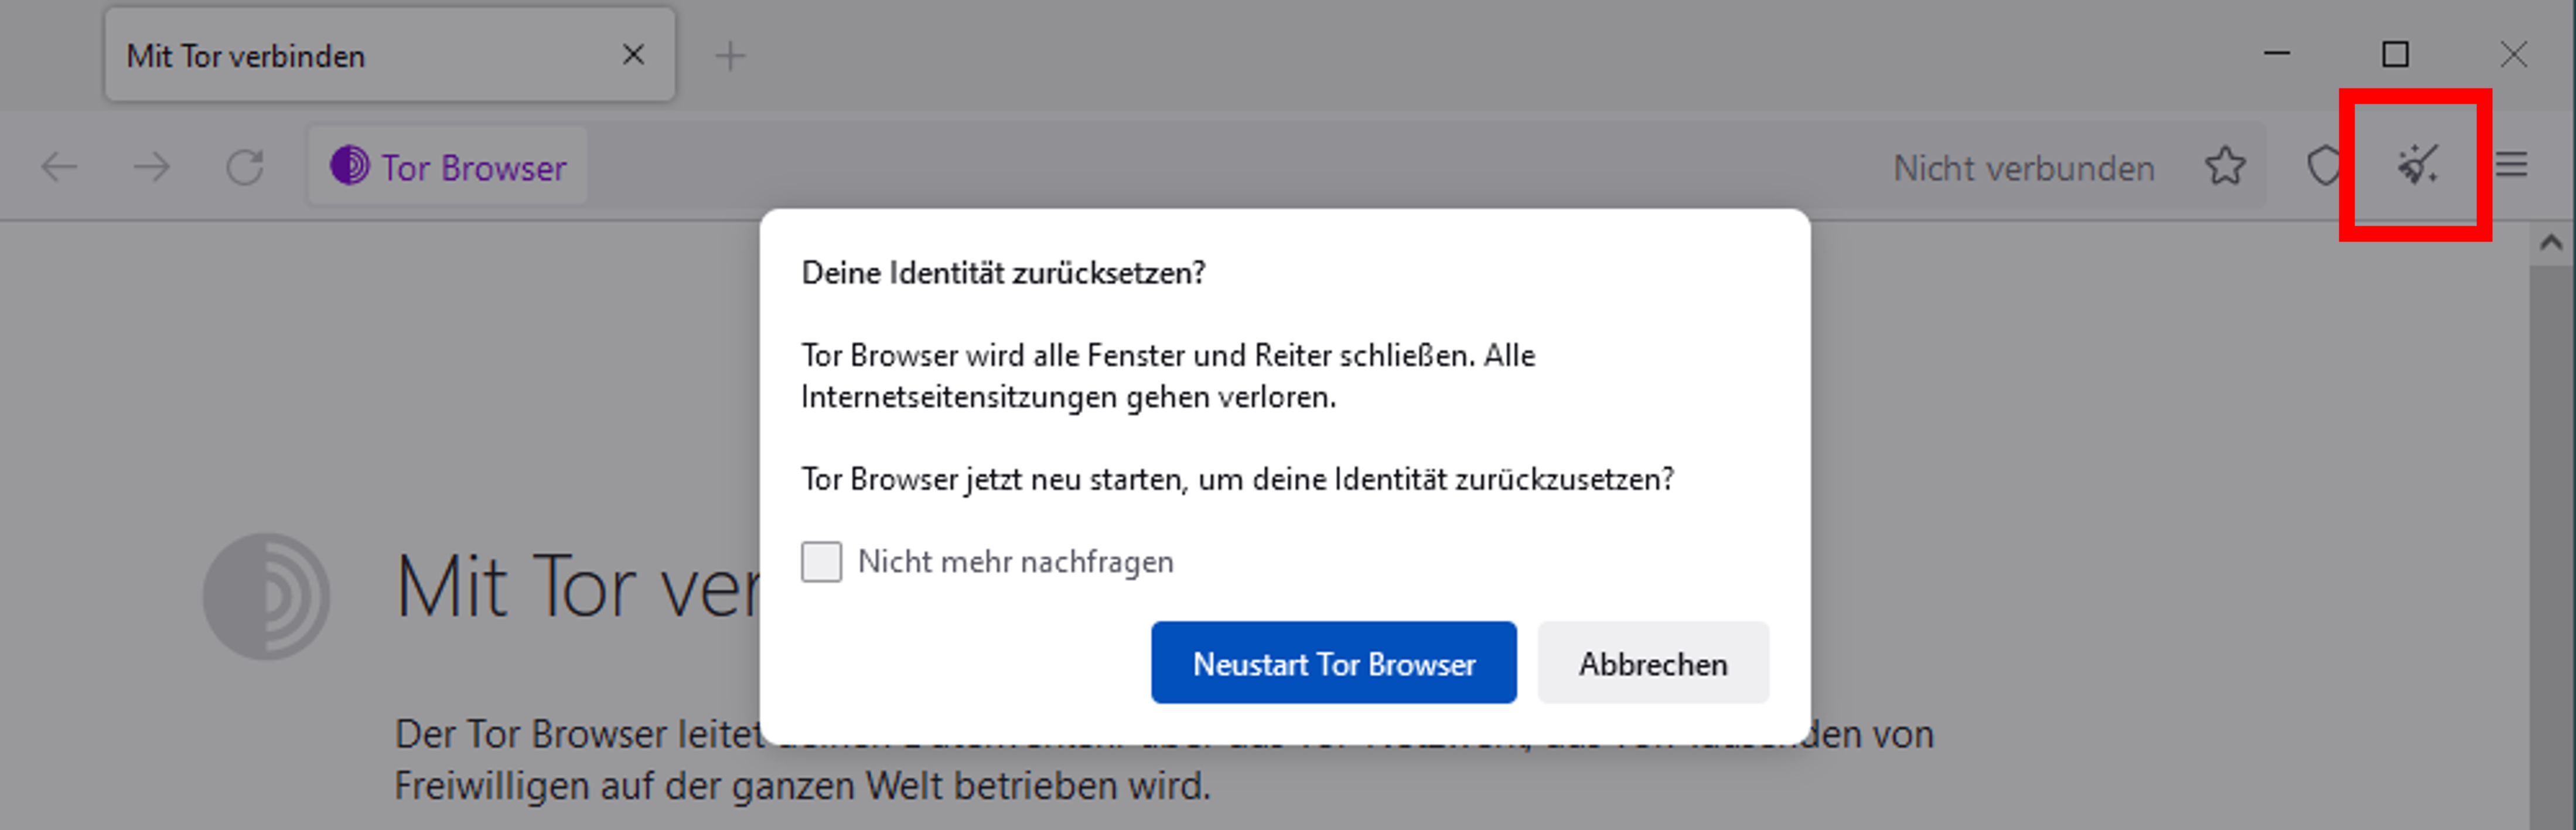
\includegraphics{bilder/tor-new-identity.png}}
%	\label{...}
	\caption{Tabelle mit wiederherstellbaren Dateien: Logfile 1 vs. Logfile 2}
\end{figure}
Die Funktion "Neue Identität" im Tor Browser ermöglicht es, alle aktuellen Tabs und Fenster zu schließen, sämtliche private Informationen wie Cookies und Verlauf zu löschen und für alle Verbindungen neue Relays zu verwenden.

Für diesen Versuch: Tor Version 12.0.4 (64 Bit)

\subsubsection*{Chrome}

\subsubsection*{Brave}

\subsection{Browsing Szenario}

% > Image als Hex: \cite{Ohana.2013}

Siehe Ziel der Arbeit: Versuch soll nicht Situation eines Ermittlers simulieren, der eine unbekannte Datenlage hat.
Stattdessen: Bereits vor Analyse bekannt, nach welchen Daten gesucht werden muss.

Deshalb wird für Versuch definiert, mit welchen Daten der Rechner kontaminiert werden soll.

Im Falle der Browser-Forensik wird dazu ein sog. "Browsing Szenario" festgelegt. (TODO: Quelle, alternative Namen).

Dabei handelt es sich um Reihe von fest definierten Aktivitäten, die für jeden zu untersuchenden Browser durchgeführt werden.

Anforderungen an Browsing Szenario 
- Ziel: PB Artefakte, die ausschließlich in Browsing-Szenario vorkommen, bspw. "twitter" oder "facebook" bereits in vielen Windows-Standardanwendungen enthalten.
- (TODO: Literatur)

Folgende Schritte werden in jedem Browser durchgeführt: 

\begin{enumerate}
\item  www.google.com aufrufen
	\begin{enumerate}[label*=\arabic*.]
	\item Alle Cookies akzeptieren 
	\item Google-Suche nach "pfaffenhofen"
	\end{enumerate}
\item www.google.com aufrufen
	\begin{enumerate}[label*=\arabic*.]
	\item Cookies alle akzeptieren 
	\item Google-Suche nach "nanoradar" 
	\end{enumerate}
\item www.google.com aufrufen
	\begin{enumerate}[label*=\arabic*.]
	\item Cookies alle akzeptieren 
	\item Google-Suche nach "mallofamerica"
	\item Auf Suchergebnis "mallofamerica.com" klicken
	\end{enumerate}
\item www.google.com aufrufen
	\begin{enumerate}[label*=\arabic*.]
	\item Cookies alle akzeptieren 
	\item Google-Suche nach "mooserliesl"
	\item Auf Suchergebnis "mooserliesl.de" klicken
	\end{enumerate}
\item "www.unitree.com" über URL-Leiste öffnen
\item "www.donaukurier.de" über URL-Leiste öffnen
	\begin{enumerate}[label*=\arabic*.]
	\item Donaukurier Logo in neuem Tab öffnen
	\end{enumerate}
\item "mail.google.com" über URL-Leiste öffnen
	\begin{enumerate}[label*=\arabic*.]
	\item Mit google Account anmelden: 
			\begin{enumerate}[label*=\arabic*.]
			\item E-Mail = "computerforensikvl@gmail.com"
			\item Passwort = "Vorlesung23!"
			\end{enumerate}
	\item Neue E-Mail schreiben:
			\begin{enumerate}[label*=\arabic*.]
			\item Empfänger: "cas0597@thi.de" und "chs3702@thi.de"
			\item Betreff: "Betrefftext"
			\item Mailinhalt: "Mailinhalt"
			\end{enumerate}			
	\end{enumerate}
\end{enumerate}

Aus diesem Browsing-Szenario lassen sich sogenannte "private Browsing Artefakte", kurz PB Artefakte ableiten.
Wie in Kapitel X (TODO!) beschrieben, handelt es sich dabei um Strings oder reguläre Ausdrücke, die eindeutig einem Schritt im Browsing-Szenario zugeordnet werden können.
PB Artefakte in Tabell X (TODO!) beschrieben.

Bemerkung: "mail.google.com" nicht aufgeführt, da festgestellt, dass URL bereits in vielen Windows Standardanwendungen enthalten ist.

\begin{table}[]
\begin{tabular}{|c|l|c|}
\hline
\textbf{Kategorie}           & \multicolumn{1}{c|}{\textbf{Private Browsing Artefakt}}                                      & \textbf{\begin{tabular}[c]{@{}c@{}}Schritt im\\  Browsing Szenario\end{tabular}} \\ \hline
\multirow{4}{*}{Suchbegriff} & "pfaffenhofen"                                                                               & 1.2                                                                              \\ \cline{2-3} 
                             & "nanoradar"                                                                                  & 2.2                                                                              \\ \cline{2-3} 
                             & "mallofamerica"                                                                              & 3.2                                                                              \\ \cline{2-3} 
                             & "mooserliesl"                                                                                & 4.2                                                                              \\ \hline
\multirow{4}{*}{URL}         & "mooserliesl.de"                                                                             & 3.3                                                                              \\ \cline{2-3} 
                             & "mallofamerica.com"                                                                          & 4.3                                                                              \\ \cline{2-3} 
                             & "unitree.com"                                                                                & 5.                                                                               \\ \cline{2-3} 
                             & "donaukurier.de"                                                                             & 6.                                                                               \\ \hline
Bild                         & \begin{tabular}[c]{@{}l@{}}0x89 0x50 0x4E 0x47 ...\\ (PNG als Hexadezimalwerte)\end{tabular} & 6.1                                                                              \\ \hline
\multirow{4}{*}{E-Mail}      & "computerforensikvl@gmail.com"                                                               & 7.1.1                                                                            \\ \cline{2-3} 
                             & "Vorlesung23!"                                                                               & 7.1.2                                                                            \\ \cline{2-3} 
                             & "cas0597@thi.de"                                                                             & 7.2.1                                                                            \\ \cline{2-3} 
                             & "chs3702@thi.de"                                                                             & 7.2.1                                                                            \\ \hline
\end{tabular}
\end{table}


\subsection*{VM Konfiguration}

Best Practice in Browser Forensik: Versuche sowie Analysen in virtualisierter Umgebung durchführen. (TODO: Quellen)
- Dadurch Reproduzierbarkeit der Ergebnisse sichergestellt
- Keine Vermischung der PB Artefakte, wenn gleicher Rechner verwendet
- Keine Vermischung der Versuchsumgebung mit der Analyseumgebung
- Ergebnisse sind transportabel -> Zustände von Virtuellen Maschinen exportierbar
- Deshalb oft in Literatur empfohlen

Als Virtualisierungssoftware für Versuch verwendet: Kostenlose Oracle VirtualBox VM, Version 7.0.8 r156879 (Qt5.15.2)

In Literatur zu Browserforensik empfohlen: pro Browser eine VM erstellen, auf der Browsing Szenario durchgeführt wird.

Daui zunächst eine Benchmark-VM erstellt. Wird nach Basiskonfiguration als OVA exportiert und für jeden Browser dupliziert. Anschließend für jede VM entsprechenden Browser installiert.

\paragraph*{Betriebssystem}
VM Betriebssystem: In den 23 untersuchten wissenschaftlichen Veröffentlichungen wurden die privaten Browsermodi ausschließlich unter Windows untersucht.
Da Ziel dieser Arbeit ist keine neuen wissenschaftlichen Ergebnisse: Für diesen Versuch Windows 10 verwendet.
Deshalb auf VM installiert: Windows 10 Pro, Build: 19045.2006, nicht aktiviert

\paragraph*{Speicher}
In Literatur keine Angaben über empfohlene Festplattengrößen.
Deshalb an Microsoft Empfehlungen orientiert: VM erhält 30 GB (VDI-Format) Festplatte, kein SSD-Laufwerk
% https://support.microsoft.com/en-us/windows/windows-10-system-requirements-6d4e9a79-66bf-7950-467c-795cf0386715
In Literatur ebenfalls kaum Angaben über empfohlene RAM Größe gemacht:
> Wichtige Entscheidung, da wie später in Kapitel X beschrieben, RAM-Größe Auswirkungen auf Ergebnisse hat
> Rochmadi et al.: 2 GB \cite{Rochmadi.2017}
> Ohana et al.: 4 GB \cite{Ohana.2013}: 
> Hier: mit 6 GB die maximal mit verfügbaren Speicherresourcen auf Analyserechner mögliche Größe gewählt, um später Speicherabbilder des Arbeitsspeichers zu sichern.

\paragraph*{Netzwerkkonfiguration}
VM wurde mittels Netzwerkbrücke direkt mit dem physischen Netzwerk des Hostsystems verbunden. Somit erhält jede virtuelle Maschine eine eigene IP-Adresse im Netzwerk des Rechners, auf dem die VM läuft.
Der Netzwerkadapter der VM wurde erst nach Browserinstallation aktiviert, um eine versehentliche Kontaminierung der VM zu vermeiden.

\subsubsection*{Installierte Programme auf VM}
Um Programme auf VM zu installieren: Gemeinsamer Order zwischen VM und Rechner eingerichtet, auf dem VM läuft. Ordner wird in VM als Netzwerklaufwerk angezeigt
Grund: VM erst mit Beginn von Browsing Szenario mit Netzwerk und Internet verbinden. Deshalb: Programme mussten auf Rechner auf dem VM läuft heruntergeladen werden und über gemeinsamen Order auf VM transportiert werden.

\paragraph*{Browserinstallation}
Zunächst Browser installiert. Folgende Installationsverzeichnisse verwendet:
\begin{enumerate}
\item[\textbf{Firefox}] \texttt{C:\\Program Files\\Mozilla Firefox\\firefox.exe}
\item[\textbf{Tor}] \texttt{C:\\Program Files\\Tor Browser\\Browser\\firefox.exe}
\item[\textbf{Chrome}] ***TODO!***
\item[\textbf{Brave}] ***TODO!***
\end{enumerate}

Weiterhin wurden zwei Werkzeuge der Sysinternal-Abteilung von Microsoft installiert: "Process Monitor" und "Process Explorer". 
Hintergrund: siehe Ziel der Arbeit: ersuch soll nicht Situation eines Ermittlers simulieren, der eine unbekannte Datenlage hat. Mithilfe der Tools soll Browserverhalten während des Szenarios aufgezeichnet und untersucht werden können.

\paragraph*{Process Monitor}
Process Monitor ermöglicht die Aufzeichnung aller Aktivitäten und Ereignisse, die auf einem Windows-System im Zusammenhang mit Prozessen, Dateisystemen, Registrierungseinträgen und Netzwerkverbindungen stattfinden. Die Aufzeichnung kann als "Process Monitor Logfile" (PML) exportiert werden. Die aufgezeichneten Aktivitäten können somit beliebig gefiltert werden, beispielsweise nach Prozessnamen oder Operation, die der Prozess durchgeführt hat. Die Möglichkeit zum Export als CSV-Datei ermöglicht eine umfassende Untersuchung mit weitern Programmen, wie Microsoft Excel.
% https://learn.microsoft.com/de-de/sysinternals/downloads/procmon
Für diesen Versuch verwendet: Version 3.93

\paragraph*{Process Explorer}
Weiterhin wurde "Process Explorer" installiert. Das Tool erweitert die Funktionen des Windows Task Managers und ermöglicht es, einen umfassenden Überblick über alle aktiven Prozesse und deren Eigenschaften zu erhalten. Beispielsweise können alle ausgeführten Windows Dienste mit ihren PIDs angezeigt werden.
% https://learn.microsoft.com/de-de/sysinternals/downloads/process-explorer
Für diesen Versuch verwendet: Version 17.04

\subsection{Analysewerkzeuge}

Neben Konfiguration der VM muss Analyseumgebung vorbereitet werden.
Als Analyseumgebung dient der Rechner, auf dem die VM läuft.
Spezifikationen: *** TODO ***
Dazu: Diverse Tools zur Analyse installieren

\subsubsection*{Autopsy}
Wie im nächsten Kapitel X (TODO!) beschrieben, müssen Festplattenabbilder untersucht werden.
Dazu wird in der Literatur das Tool "Autopsy" empfohlen.

Autopsy ist ein Open-Source-Digital-Forensik-Tool, das auf der Sleuthkit-Bibliothek basiert. 
Sleuthkit ist eine Sammlung von Open-Source-Tools für die forensische Analyse von Dateisystemen. Es bietet Funktionen zum Lesen, Analysieren und Wiederherstellen von Daten aus verschiedenen Dateisystemen. 
Autopsy baut auf der Funktionalität von Sleuthkit auf und bietet eine grafische Benutzeroberfläche für die forensische Analyse. 
Wurde hauptsächlich in Java geschrieben.
Es erweitert die Funktionalität von Sleuthkit, indem es zusätzliche Tools, Plug-Ins und Automatisierungsfunktionen bereitstellt, um den forensischen Untersuchungsprozess zu unterstützen.
 
Für diesen Versuch verwendet: Version 4.20.0

\subsubsection*{Volatility}
Neben der Analyse von Festplattenabbildern müssen gemäß Kapitel X Abbilder des Arbeitsspeichers unteruscht werden. Dazu wird das in der Literatur empfohlene Tool "Volatility" verwendet.
 
Das Volatility Memory Forensics Framework ist ein Open-Source-Tool, das für die forensische Analyse von Arbeitsspeicherabbildern verwendet wird. Es ist speziell darauf ausgerichtet, Informationen und Artefakte aus dem physischen oder virtuellen Arbeitsspeicher eines Computers zu extrahieren.

Geschrieben in Python, frei auf GitHub verfügbar:	
Version: Volatility3, Version 2.4.1 (aktuellster Release)

Für diesen Versuch verwendet: "Volatility3"
= vollständige Neuschreibung des Volatility Memory Forensics Frameworks, die im Jahr 2020 veröffentlicht wurde. Behebt technische und Performanceprobleme der vorherigen Version.

Oft beworbender Vorteil von Volatility3: kein "Profile" mehr notwendig. Volatility3 erstellt Symboltabellen für Windows-Speicherabbilder basierend auf dem Speicherabbild selbst.
Dabei handelt es sich um ein Konfigurationseinstellung, welche die Speicherstruktur und die Verhaltensweisen des Betriebssystems definiert.
	% https://volatility3.readthedocs.io/en/latest/vol2to3.html
	% https://www.volatilityfoundation.org/
	% https://github.com/volatilityfoundation/volatility3

Volatility basiert auf Plugins, welche spezifische Funktionen und Analysen für verschiedene Aspekte des Systems bereitstellen. Für diesen Versuch werden folgende Plugins verwendet. 
\begin{itemize}
\item pslist	
\item yarascan		
\item memmap	 	
\item filescan
\item svcscan
\end{itemize}
		
Genaue Beschreibung der PlugIns und deren Zusammenhang: Siehe Analysephase in Kapitel X (TODO!).

\subsection*{Übersicht verwendete Software}

Tabelle X listet zusammenfassend alle in diesem Versuch verwendeten Software-Programme, deren Zweck sowie Version auf.

Neben den Programmen zur Analyse der Speicherabbilder: diverse zusätzliche unterstützende Tools zur vollständigen Analyse benötigt, diese werden nicht genauer beschrieben.
- Nur in Tabelle aufgenommen

\begin{table}[]
\resizebox{\linewidth}{!}{
\begin{tabular}{|l|l|l|}
\hline
\multicolumn{1}{|c|}{\textbf{Software}} & \multicolumn{1}{c|}{\textbf{Zweck}}                                              & \multicolumn{1}{c|}{\textbf{Version}} \\ \hline
Oracle VirtualBox                       & Virtualisierung                                                                  & 7.0.8 r156879                         \\ \hline
Windows 10 Pro                          & VM Betriebssystem                                                                & Build: 19045.2006                     \\ \hline
Process Monitor                         & Aufzeichnung Prozessaktivitäten                                                  & 3.93                                  \\ \hline
Process Explorer                        & Darstellung der Eigenschaften aktueller Prozesse                                 & 17.04                                 \\ \hline
Autopsy                                 & Analyse Festplattenabbilder                                                      & 4.20.0                                \\ \hline
Volatiltiy                              & Analyse RAM-Abbilder                                                             & Volatility3 Version 2.4.1             \\ \hline
HxD                                     & Analyse Binärdateien in hexadezimaler und ASCII-Darstellung                      & 2.5.0.0                               \\ \hline
Notepad++                               & Analyse strukturierter Dateiformate, z.B. JSON, XML                              & 8.4.5                                 \\ \hline
Registry Explorer                       & Grafischer Oberfläche zur Untersuchung von Windows-Registry Hives                & 2.0.0.0                               \\ \hline
DB Browser for SQLite                   & Grafische Oberfläche zur Verwaltung und Untersuchung von SQLite-Datenbanken      & 3.12.2                                \\ \hline
sqldiff.exe                             & Befehlszeilen-Programm zur Anzeige von Unterschieden zwischen SQLite-Datenbanken & 3.42.0                                \\ \hline
ChromeCacheView                         & Einlesen von Chrome Cache-Dateien und visuelle Aufbereitung des Inhalts          & 2.46                                  \\ \hline
MZCacheView                             & Einlesen von Firefox Cache-Dateien und visuelle Aufbereitung des Inhalts         & 2.21                                  \\ \hline
FirefoxCache2                           & Erweitert MZCacheView, um Firefox "index"-Cachedatei zu analysieren              & Commit b50ab4f                        \\ \hline
dejsonlz4                               & Dekomprimierung von .jsonlz4-Dateien                                             & Commit c4305b8                        \\ \hline
\end{tabular}
}
\end{table}



\section{Datensammlung}

*** TODO: Schreiben, dass für diesen Versuch auch VM-Snapshots zu bestimmten Zeitpunkten aufgetaut werden können ***

In der Phase der Datensammlung werden alle potenziellen Beweismittel identifiziert, gesammelt. Ziel ist es, die Daten in einem Format zu sammeln, in dem sie in der nächsten Phase analysiert werden können. \cite{Izzati.2022}

Für diesen Versuch umfasst dies die Durchführung des Browsing Szenarios sowie die Sammlung von Ressoucen, die potentielle private Browsing Artefakte enthalten.

\subsection*{Process Monitor Logfiles}
Gemäß dem in Kapitel X definierten Ziel der Arbeit wird der Versuch wird nicht aus Sicht eines Forensikers durchgeführt, der nur begrenzten Zugriff auf Beweismittel hat. 
Stattdessen soll mit diesem Versuch das Verhalten von privaten Browsingmodi möglichst vollständig untersucht werden, mit dem Ziel alle auf der VM hinterlassenen privaten Browsing Artefakte zu identifizieren.
Den gleichen Ansatz verfolgten Fayyad-Kazan et al. \cite{Fayyad.2021} Sie schlagen deshalb vor, alle Aktivitäten des Browsers während Browsing-Szenarios aufzeichnen.
Sie empfehlen dazu das oben in Kapitel X beschriebene Tool "Process Monitor".
Mithilfe einer grafischen Oberfläche können die aufgezeichneten Aktivitäten als Process Monitor Logfile sowie CSV Datei gespeichert werden.
Nach Empfehlung der Autoren liegt bei den Browseraktivitäten der Fokus auf Schreibaktivitäten im Dateisystem sowie geänderte Werte in der Registry. \cite{Fayyad.2021, Rochmadi.2017}
Um die aufgezeichneten PML-Dateien auf den Analyserechner zu transportieren, wird der bereits in Kapitel X zur Installation von Programmen verwendete gemeinsame Ordner verwendet.

\subsection*{Speicherabbilder}
Eine der Hauptaufgaben eines Computer-Forensischen-Ermittlers ist die Erstellung und Analyse von Speicherabbildern. \cite{Hassan.2019}
Dabei handelt es sich um eine direkte Kopie der Daten auf den Speichermedien des Rechners. \cite{Hassan.2019}
Dazu zählen beispielsweise Festplatten, der Arbeitsspeicher sowie angeschlossene Speichermedien wie USB-Sticks.
Zur Identifikation von Artefakten auf dem untersuchten Rechner muss vermieden werden, auf den originalen Speichermedien zu arbeiten.
Dadurch können Beweise verfälscht werden und nicht mehr vor Gericht verwendet werden. \cite{Hassan.2019}
Aus diesem Grund muss es sich bei den analysierten Speichermedien stets um Abbilder ("Images"), also Kopien des originalen Mediums handeln.

Im Falle der Browser Forensik werden in der Literatur zwei Arten von Speichermedien untersucht: Festplatten (TODO: Alle Quellen) und der Arbeitsspeicher (TODO: Alle Quellen)

\paragraph*{Festplatten-Image}
Um ein Abbild einer phsysikalische Festplatten zu erstellen gibt es diverse Software- und Hardware Lösungen. 
Da in diesem Versuch die Festplatten virtualisiert wurden, entspricht ein Festplatten-Abbild einem sogenannten "VM-Snapshot".
Dabei handelt es sich um eine Momentaufnahme von einer virtuellen Maschine. Ein Snapshot erfasst den Arbeitsspeicher, den Prozessorzustand sowie den Festplatteninhalt zu einem bestimmten Zeitpunkt. % https://docs.oracle.com/en/virtualization/virtualbox/6.0/user/snapshots.html
Bei Oracle VirutalBox kann eine VM Snapshot über die grafische Oberfläche durchgeführt werden.
Dazu wird ausgehend vom letzten beziehungsweise aktuellen Zustand der VM im Menü "Sicherungspunkte" die Option "Erzeugen" ausgewählt.
\begin{figure}[h!]
	\resizebox{\linewidth}{!}{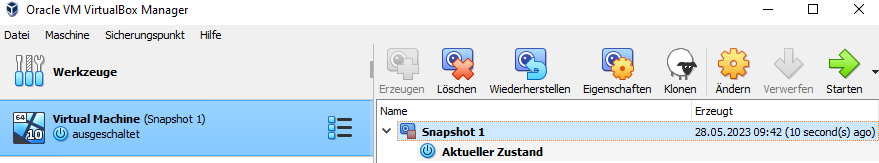
\includegraphics{bilder/snapshot2.png}}
%	\label{...}
	\caption{TODO}
\end{figure}
Dies kann sowohl im an- und ausgeschaltetem Zustand der virutellen Maschine durchgeführt werden. Somit kann ein VM-Snapshot sowohl zur Live- als auch Post-Mortem-Forensik verwendet werden.
Durch den Snapshot wird ein "Virtual Disk Image", eine VDI-Datei, im Snapshot-Ordner der VM erzeugt. Diese Laufwerksdatei enthält nur differentielle Daten zum vorherigen Snapshot bzw. zum aktuellen Zustand, wenn es sich um den ersten Snapshot handelt. Die Datei ist meist wenige KiloByte groß.
Um aus den differentiellen Daten ein vollständiges Festplatten-Image zu erzeugen muss aus dem Snapshot über die Option "Klonen" eine eigenständige VM erstellt werden. 
Dabei muss die Option "vollständiger Klon" ausgewählt werden. Die VDI-Datei der geklonten VM enthält alle Festplatten-Daten zum Zeitpunkt des durchgeführten Snapshots.

Wie einleitend beschrieben, müssen die in dieser Phase gesammelten Daten in einem Format vorliegen, das in der Analysephase verwendet werden kann.
Wie im nächsten Kapitel beschrieben, werden die Festplatten-Images mit dem Tool Autopsy analysiert.
Da Autopsy kein VDI-Format unterstützt, müssen die Laufwerksdateien der geklonten Snapshots in ein das Image-Format (.img) umgewandelt werden.
Dabei handelt es sich um ein generisches Dateiformat, welches ein binäres Abbild des Speichermediums speichert. 
Oracle VirtualBox bietet das in der Installation enthaltene Befehlszeilen-Tool "vboxmanage" für diese Dateiumwandlung an. Mit dem Befehl \texttt{vboxmanage clonehd <VDI\_File>.vdi <IMG\_File>.img --format raw} wird das VirtualBox Disk Image "VDI\_File" in die Image-Datei "IMG\_File" umgewandelt.

*** TODO: Hier Einlesen der Festplatten-Images => Zeitaufwändig! ***

\paragraph*{RAM-Dump}

Wie oben beschrieben, enthält ein VM-Snapshot neben dem Festplatteninhalt den Inhalt des Arbeitsspeichers zum Zeitpunkt der Momentaufnahme.
Ein sogenannter "RAM-Dump" erfasst den genauen Zustand des Arbeitsspeichers, einschließlich der im Speicher befindlichen Daten, Programme und Prozesse.
Der RAM-Dump eines Snapshots wird neben weiteren Daten in .sav Dateien gespeichert. 
VirtualBox bietet aktuell keine Möglichkeit aus diesen Dateien den RAM in einem analysierbaren Format zu extrahieren.
% https://kollee.github.io/posts/memory-forensics-of-a-virtualbox-vm/
Stattdessen wird von VirtualBox empfohlen, Abbilder des Arbeitsspeichers ebenfalls über das "vboxmanage" Befehlszeilen-Tool durchzuführen.
Im Unterschied zu Festplatten-Images, können RAM-Dumps ohne zusätzliche Hardware damit nur in angeschaltetem Zustand der virtellen Maschine durchgeführt werden. 
Um ein Abbild des Arbeitsspeichers einer laufenden virtuellen Maschine zu erstellen wird folgender Befehl ausgeführt: \texttt{vboxmanage debugvm <VM Name> dumpvmcore --filename "<RAM Dump Dateiname>.elf}. Zur Analyse des RAM-Dumps ist keine weitere Verarbeitung notwendig. RAM-Dumps im .elf Format können direkt vom Analysetool Volatility eingelesen werden.		

\paragraph*{Zeitpunkte zur Datensammlung}
Wichtig für die qualität der Versuchsergebnisse ist das Festlegen der Zeitpunkte im Browsing Szenario zum Sammeln der Daten.
Dieses Thema wird in der Literatur kaum thematisiert. Die Autoren wählen die Zeitpunkte meist ohne Begründung.
Ausschließlich Fayyad et al. geben an, dass sie die Process Monitor Logfiles während des Browsing Szenarios erstellten. Einen präzisen Start- und Endzeitpunkt der Aufnahme nennen sie nicht.
Abbilder des Arbeitsspeichers werden bei 23 Untersuchten Papern am häufigsten nach Durchführung des Browsing Szenarios und Schließen des Browsers durchgeführt \cite{Hariharan.2022, Izzati.2022, Md.2018, Ohana.2013}. Mahlous et al. erstellen einen RAM-Dump mit geöffnetem Browser, jedoch keinen nach Schließen des Browsers \cite{Mahlous.2020}.
Rochmadi et al. erstellen mehrere RAM-Dumps zu unterschiedlichen Zeitpunkten: Vor dem Schließen des Browser, nach dem Schließen des Browsers sowie nach dem Löschen der Registry \cite{Rochmadi.2017}
Festplattenabbilder werden am häufigsten im Zuge der Post-Mortem-Forensik analysiert und nach Herunterfahren der VM gesichert \cite{Fayyad.2021, Mahlous.2020, Horsman.2019, Md.2018, Gabet.2018, Montasari.2015, Chivers.2014, Ohana.2013}.
In einigen Fällen wurde gar nicht erwähnt, zu welchen Zeitpunkten im Browsing Szenario die Daten gesammelt wurden \cite{Sajan.2021, Nalawade.2016, Montasari.2015, Satvat.2014, Said.2011, Aggarwal.2010}.

Dieses Problem haben Muir, Leimich und Buchanan erkannt und Zeitpunkte zur Datensammlung vorgeschlagen, um das Browserverhalten während des Browsing-Szenarios vollständig zu überwachen und zu analysieren. Wie in Abbildung X (TODO!) dargestellt, wurde sich an diesen Zeitpunkten für diesen Versuch orientiert.
\begin{figure}[h!]
	\centering
	\small
	\centerline{\resizebox{\linewidth}{!}{\input{bilder/datensammlung-zeitpunkte-Latex.pdf_tex}}}
	\caption{Datensammlung Zeitpunkte}
	\label{fig:jes}
\end{figure}
Nach der Browser-Installation, vor Beginn des Browsing-Szenarios wird der erste RAM-Dump sowie der erste VM-Snapshot erstellt.
Diese Speicherabbilder dienen als Benchmark für die Analyse, da in diesen Speicherabbildern kein PB Artefakt gefunden werden darf.

Nachdem der Private Modus im Browser geöffnet wird, bevor das Browsing Szenario beinnt wird die Aufnahme des ersten Process Monitor Logfiles gestartet.
Die Aufzeichnung beginnt erst zu diesem Zeitpunkt, da beim erstmaligem Öffnen der Browser einige Dateien initial angelegt werden. Um ausschließlich Schreiboperationen aufzuzeichnen, die auf das private Browsing zurückzuführen sind, wird die Aufzeichnung erst nach dem erstmaligen Öffnen des Browsers im privaten Modus gestartet.

Nach Durchführung des Browsing-Szenarios, während der Browser noch geöffnet ist, wird die Aufnahme des ersten Process Monitor Logfiles beendet. Weiterhin wird ein zweiter RAM-Dump sowie VM-Snapshot erstellt. Anschließend wird das eine zweite Process Monitor Aufzeichnung gestartet. 
Somit enthält das erste Logfile zu diesem Zeitpunkt die Prozessaktivitäten während des Browsing Szenarios. 

Nachdem der Browser geschlossen wurde, wird die Aufzeichnung des zweiten Process Monitor Logfiles beendet. Zusätzlich wird ein dritter RAM-Dump sowie  VM-Snapshot erstellt. Somit enthält das zweite Logfile wird alle Prozessaktivitäten vom Schließen der Browsers.

Nach Herunterfahren der VM wird ein vierter VM-Snapshot erstellt, der für die für Post-Mortem Analyse relevant ist.

\paragraph*{Sonderfälle}

Dieses Vorgehen zur Datensammlung wird bei allen Browsern durchgeführt. Einzig der Tor-Browser weicht davon ab. Wie in Kapitel X beschrieben, besitzt der Tor-Browser die Funktion der "Neuen Identität", eine Funktion um bestimmte Nutzerdaten zu löschen und zurückzusetzen.
% https://support.torproject.org/de/glossary/new-identity/
Um diese Funktion in das Browsing Szenario aufzunehmen, werden beim Tor-Browser zusätzlich Daten vor und nach der Erstellung einer "Neuen Identiät" gesammelt. Wie in Abbildung X (TODO!) dargestellt, umfasst dies einen zusätzlichen RAM-Dump sowie VM-Snapshot und ein weiteres Process Monitor Logfile.
\begin{figure}[h!]
	\centering
	\small
	\centerline{\resizebox{\linewidth}{!}{\input{bilder/datensammlung-zeitpunkte-tor-Latex.pdf_tex}}}
	\caption{Datensammlung Zeitpunkte Tor}
	\label{fig:jes}
\end{figure}
	
Bei Durchführung des Browsing-Szenarios für den Firefox-Browser wurde nach erstmaligem Öffnen des Browsers automatisch die Webseite \texttt{https://www.mozilla.org/de/privacy/firefox/} geöffnet. Zu diesem Zeitpunkt befand sich Firefox nicht im privaten Modus. Bei der automatisch geöffneten Seite handelt es sich um Hinweise zum Datenschutz beim Firefox- Browser.

\section{Datenanalyse}

Nachdem Daten in Form von Process Monitor Logfiles und Festplatten- sowie RAM-Speicherabbildern gesammelt: Daten analysieren.

Analyse heißt bei Browser Forensik: Suchen nach PB Artefakten aus Browsing Szenario in gesammelten Daten
 = Suchen nach Strings in Tabelle X aus Kapitel X (TODO!), der einem konkreten Schritt im Browsing Szenario entspricht.

Wichtig dabei: gefundenes Artefakt muss eindeutig Browser zugeordnet werden können.
Oft kritisiert: Viele Autoren (TODO: Quellen) verlassen sich beispielsweise bei der Analyse der RAM-Dumps auf eine einfache Stringsuche in einem Hexadezimal-Editor.
Sagt jedoch nichts darüber aus, ob gefundener String tatsächich auf privates Browsen zurückzuführen ist.
*** TODO: String in Editor Beispiel ***

Mit dieser Anforderung lassen sich die gesammelten Daten des Versuchs in drei Kategorien aufteilen:
> Common Locations
> Uncommon Locations	
> Registry

\subsection{Common Locations}

*** TODO: Wichtig: NUR FESTPLATTE, NICHT RAM ***

Die sogenannten "Common Locations", (dt. "gängige Speicherorte") beziehen im Zusammenhang der Browserforensik auf die standardmäßigen Verzeichnisse eines Browsers. 
Dazu zählen beispielsweise Ordner von Browsern zur Verwaltung von Nutzerdaten.

Untersucht werden Common Locations mittels "Whitebox-Analyse" \cite{Bonetti.2014}
Der forensische Analyst besitzt dabei über umfassende Kenntnisse über den Browser und hat vollständigen Zugriff auf das untersuchte System. 
Der Fokus liegt darauf, das System vollständig zu verstehen und alle relevanten Beweise zu sammeln.
Dazu werden zuerst die gängigen Browser-Speicherorte identifiziert. 
Im Falle dieses Versuchs werden die Browser Speicherorte über die Schreiboperationen der Process Monitor Logfiles identifiziert.
Anschließend wird für jede Datei in den Speicherorten geprüft, ob PB Artefakte enthalten sind.
Dazu sind zwei Schritte notwendig:
\begin{enumerate}
\item Dateiextraktion: Extrakion der Datei aus dem Speicherabbild. Wenn die Datei nicht mehr vorhanden ist, werden dazu ggf. Tools zur Dateiwiederherstellung benötigt.
\item Dateianalyse: Um zu überprüfen ob die Datei PB Artefakte enthält, werden ggf. Tools für spezielle Dateiformate benötigt, beispielsweise Dekomprimierungstools.
\end{enumerate}

Die Untersuchung der Common Locations wird im Zusammenhang der Browser-Forensik auch "Triage" genannt \cite{Horsman.2019}. Wenn für den vorliegenden Browser die gängingen Speicherorte bekannt sind, kann im ersten Analyeschritt gezielt nach Dateien gesucht werden, die aus Erfahrungswerte PB Artefakte beinhalten.

\subsubsection*{Process Monitor Logfiles}

\paragraph*{Identifikation der Common Locations}
Um die gängigen Browserpfade und -dateien zu identifizieren, werden die in den Process Monitor Logfiles aufgezeichneten Schreibaktivitäten der Browserprozesse ausgewertet.

Dazu wird jede Process Logfile mit dem Process Explorer eingelesen. Anschließend werden die Aktivitäten gefiltert.
\begin{figure}[h!]
	\resizebox{\linewidth}{!}{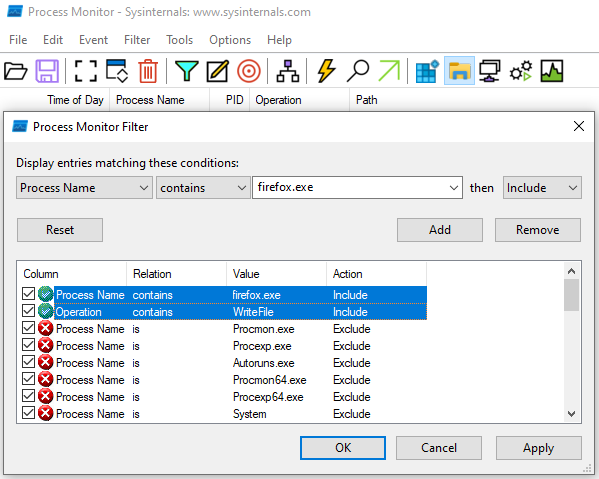
\includegraphics{bilder/process-monitor-filter.png}}
%	\label{...}
	\caption{Tabelle mit wiederherstellbaren Dateien: Logfile 1 vs. Logfile 2}
\end{figure}
Wie in Abbildung X dargestellt werden dazu ausschließlich die Option "File System Activity" ausgewählt.
Anschließend wird als Prozessname der Browserprozess gesetzt:
\begin{itemize}
\item[\textbf{Firefox}] firefox.exe
\item[\textbf{Tor-Browser}] firefox.exe und tor.exe
\item[\textbf{Chrome}] chrome.exe
\item[\textbf{Brave}] brave.exe
\end{itemize}
Weiterhin wird als Prozessoperation "WriteFile" gesetzt, um ausschließlich Schreibaktivitäten zu filtern. Hintergrund ist, dass PB Artefakte nur über "WriteFile" Operationen entstehen können, nicht über beispielsweise Löschoperationen.

Anschließend wird die gefilterte Logfile als CSV exportiert, um sie dann in Excel zu öffnen.
In Excel werden nun folgende für den Versuch irrelevante Spalten gelöscht:
\begin{itemize}
\item Time of Day: Die zeitliche Reihenfolge innerhalb einer Logfile wird nicht berücksichtigt
\item Process Name: Im Process Monitor wurde bereits nach Prozessnamen gefiltert, wordurch alle Prozesse den gleichen Prozessnamen haben.
\item Operation: Im Process Monitor bereits nach der Operation „WriteFile“ gefiltert, wodruch alle Prozesse die gleiche Operation haben
\item Result
\item Detail
\end{itemize}
Danach werden gleiche mehrfache, gleiche Operationen gelöscht.
Abschließend werden alle geschriebenen Dateien nach nach browserspezifischen Speicherorten gruppiert.

\paragraph*{Prüfung auf PB Artefakte}

Nachdem die geschriebenen Browserdateien identifiziert und kategorisiert wurden, wird für jede Datei geprüft, ob PB Artefakte enthalten sind. Die zur Dateiextraktion sowie Dateianalyse notwendigen Schritte sind in Abbildung X (TODO!) dargestellt.
\begin{figure}[h!]
	\centering
	\small
	\centerline{\resizebox{\linewidth}{!}{\input{bilder/process_monitor_to_exce-Latexl.pdf_tex}}}
	\caption{TODO: Process Monitor Write Operation to Excel Spreadsheet}
	\label{fig:jes}
\end{figure}

Zur Dateiextraktion sind werden folgende Schritte durchgeführt.
\begin{enumerate}
\item In Autopsy prüfen, ob Datei in Festplatten-Image des entsprechenden VM-Snapshots vorhanden ist. Welcher Snapshot bei welchem Logfile untersucht wird ergibt sich aus dem Browsing Szenario in Kapitel X und ist in Tabelle X dargestellt. Hier werden nur VM-Snapshots der Live-Forensik untersucht. Der vierte VM-Snapshot zählt zur Post-Mortem-Forensik und ist erst in späteren Analyseschritten relevant (siehe Kapitel X, Y, Z TODO!)
		\begin{table}[h!]
		\centering
		\begin{tabular}{l|l|l|}
		\cline{2-3}
        & Logfile     & Untersuchter Snapshot \\ \hline
		\multicolumn{1}{|l|}{\multirow{2}{*}{\begin{tabular}[c]{@{}l@{}}Firefox,\\ Chrome,\\ Brave\end{tabular}}} & Logfile 1   & Snapshot 2            \\ \cline{2-3} 
		\multicolumn{1}{|l|}{}                                                                                    & Logfile 2   & Snapshot 3            \\ \hline
		\multicolumn{1}{|l|}{\multirow{3}{*}{Tor}}                                                                & Logfile 1   & Snapshot 2            \\ \cline{2-3} 
		\multicolumn{1}{|l|}{}                                                                                    & Logfile 2-1 & Snapshot 3-1          \\ \cline{2-3} 
		\multicolumn{1}{|l|}{}                                                                                    & Logfile 2-2 & Snapshot 3-2          \\ \hline
		\end{tabular}
		\end{table}
\item Wenn ja, Datei mit Autopsy extrahieren.
\item Wenn nein, prüfen, ob Datei in Arbeitsspeicher vorhanden. Dazu wird die Ausgabe des Volatiltiy Plugins "filescan" angewendet auf den entsprechenden RAM-Dump überprüft. Dazu wird der Befehl \texttt{vol.py -f ram\_dump.img windows.filescan > filescan.txt} ausgeführt. Die Ausgabe von Filescan enthält eine Liste von Dateinamen, die im Speicher gefunden wurden. Welcher RAM-Dump bei welchem Logfile untersucht wird, ergibt sich aus dem Browsing Szenario in Kapitel X und ist in Tabelle X dargestellt.
		\begin{table}[h!]
		\centering
		\begin{tabular}{l|l|l|}
		\cline{2-3}
		                                                                                                          & Logfile     & Untersuchter RAM-Dump \\ \hline
		\multicolumn{1}{|l|}{\multirow{2}{*}{\begin{tabular}[c]{@{}l@{}}Firefox,\\ Chrome,\\ Brave\end{tabular}}} & Logfile 1   & RAM-Dump 2            \\ \cline{2-3} 
		\multicolumn{1}{|l|}{}                                                                                    & Logfile 2   & RAM-Dump 3            \\ \hline
		\multicolumn{1}{|l|}{\multirow{3}{*}{Tor}}                                                                & Logfile 1   & RAM-Dump 2            \\ \cline{2-3} 
		\multicolumn{1}{|l|}{}                                                                                    & Logfile 2-1 & RAM-Dump 3-1          \\ \cline{2-3} 
		\multicolumn{1}{|l|}{}                                                                                    & Logfile 2-2 & RAM-Dump 3-2          \\ \hline
		\end{tabular}
		\end{table}
Wenn eine Datei in der Ausgabe gefunden wurde, wird sie mithilfe des Volatility "dumpfiles" Plugins anhand der virtuellen Dateispeicheradresse extrahiert. Diese Abhängigkeiten zwischen den beiden Plugins ist in Abbildung X dargestellt.
		\begin{figure}[h!]
			\centering
			\small
			\centerline{\resizebox{0.8\linewidth}{!}{\input{bilder/volatility-filescan-dumpfiles-Latex.pdf_tex}}}
			\caption{Datensammlung Zeitpunkte Tor}
			\label{fig:jes}
		\end{figure}
\item Wenn Datei auch nicht im RAM gecacht ist: Prüfen, ob es um eine temporäre Datei (meistens Endung ".tmp") handelt.
\item Wenn es sich um eine temporäre Datei handelt: Wird die entsprechende Nicht-temporäre gewählt und und erneute bei Schritt 1 begonnen. Wenn beispielsweise die Datei "some-file.json.tmp" nicht existiert wird geprüft prüfen, ob die Datei "some-file.json" existiert.
\item Wenn es sich um keine temporäre Datei handelt: Datei als "nicht wiederherstellbar" markieren
\end{enumerate}

Nachdem eine Datei extrahiert werden konnte, werden folgende Schritte zur Dateianalsye durchgeführt.
\begin{enumerate}
	\setcounter{enumi}{7}
	\item Datei mit entsprechdem Tool untersuchen 
	\item Wenn Datei nicht lesbar ist: Datei mir zusätzlichem Tool vorverarbeiten. Beispielsweise werden komprimierte Dateien dekomprimiert. 
	\item In Excel-Tabelle markieren, ob die Datei private Browsing Artefakte enthält. Dabei gibt es drei Zustände: 
	\begin{itemize}
	\item leere Datei
	\item neuer (nicht-leerer) Inhalt
	\item gleichbleibender Inhalt
	\end{itemize}		
\end{enumerate}


\subsubsection*{SQLite-Datenbänke}

Eine besondere Rolle unter den Common Locations bei Browsern nehmen SQLite Datenbänke ein. 
SQLite ist eine relationale Datenbank-Engine. Sie ermöglicht das Speichern und Verwalten von Daten in einer einzigen Datei, ohne einen separaten Datenbankserver zu benötigen.
Diese Datenbänke speichern bei Browsern Nutzerinformationen wie Lesezeichen, Browserverlauf, Caches, Cookies und Erweiterungsdaten. Sie bieten einerseits Benutzern eine personalisierte Browsererfahrung und sind andereseits von forensischer Bedeutung, um Benutzeraktivitäten zu analysieren.

Aus diesem Grund werden für jeden Browser die SQLite Datenbanken aller Snapshots miteinander verglichen. 
\begin{figure}[h!]
	\centering
	\small
	\centerline{\resizebox{\linewidth}{!}{\input{bilder/sqlite-methodology-Latex.pdf_tex}}}
	\caption{TODO: Process Monitor Write Operation to Excel Spreadsheet}
	\label{fig:jes}
\end{figure}
Wie in Abbildung X dategestellt erfolt die Dateiextraktion analog zur Vorgehensweise bei den Schreiboperationen der Process Monitor Logfiles.

Um die SQLite Datenbänke zu analysieren wird jede Datenbank mit der gleichen Datenbank aus dem vorherigem Snapshot verglichen. Dazu wird das Befehlszeilentool "sqldiff.exe" verwendet, das über den Befehl \texttt{sqldiff.exe database1.sqlite database2.sqlite} Inhaltsunterschiede zwischen SQLite-Datenbanken anzeigt. Diese Unterschiede werden für jede Datei in jedem Snapshot untersucht und in einer Excel Tabelle festgehalten.

Zu jeder SQLite Datenbank gibt es normalerweise eine .sqlite-wal Datei. Dabei handelt es sich um den sogenannten "Write-Ahead Log", kurz WAL. Dort werden Datenbankänderungen vorübergehend protokollieren, bevor sie dauerhaft in die Hauptdatenbankdatei geschrieben werden. 
Um potentielle PB Artefakte im WAL zu berücksichtigen, werden die Inhalte des WAL in die SQLite Datei geschrieben. Dazu wird die .sqlite Datei mit dem Befehl \texttt{sqlite3 <Datenbank>.sqlite} über die sqlite3 Kommandozeile geöffnet, um anschließend den WAL in die Hauptdatenbank zu übertragen: \texttt{ sqlite3> PRAGMA wal\_checkpoint;}

\subsection{Uncommon Locations}

Ungewöhnliche Speicherorte beziehen sich auf Verzeichnisse, die nicht zu den gängigen Speicherorten gehören. 
Bei Festplatten-Images handelt es sich dabei meist um Dateien des Betriebssystems oder andere Festplattenbereiche, wie beispielsweise unallokierte Speicherbereiche.
Im Unterschied zu den "Common Locations" zählt zu den "Uncommon Locations" der Arbeitsspeicher.

Uncommon Locations werden mithilfe der "Blackbox-Analyse" untersucht \cite{Bonetti.2014}:
Dies umfasst die Durchsuchung des Beweismaterials ohne Vorwissen über das Browserverhalten sowie ohne Vorverarbeitung der Dateien.
Im Kontext der Browser Forensik werden dazu Stringsuchen nach PB Artefakten über die gesamten Speicherabbilder durchgeführt.
Somit wird im die Suchrichtung der "Common Locations" umgekehrt: 
Ausgangspunkt ist nicht eine Datei, die nach allen PB Artefakten durchsucht wird. 
Stattdessend wird das gesamte Speicherabbild nach einem konkreten PB Artefakt durchsucht.

Dies ist nur durch Unterstützung mit Forensik-Tools möglich. Somit wird bei der Analyse der Uncommon Locations in die Vollständigkeit der Tools vertraut.


\subsubsection*{Analyse mit Autopsy}

Bei den Common Locations wurde Autopsy ausschließlich zur Dateiextraktion genutzt. Bei den Uncommon Locations wird Autopsy als forensisches Werkzeug zur analyse der Festplatten-Images verwendet.
Dazu wird eine Stichwortsuche mit den in Tabelle X definierten PB Artefakten über das gesamte Festplatten-Image durchgeführt.

Autopsy bietet dazu eine Suchfunktion an. Wie in Abbildung X dargestellt, kann damit nach exakten Strings, Teilstrings oder regulären Ausdrücken in Dateinamen und Dateiinhalten gesucht werden kann.

\begin{figure}[h!]
	\resizebox{\linewidth}{!}{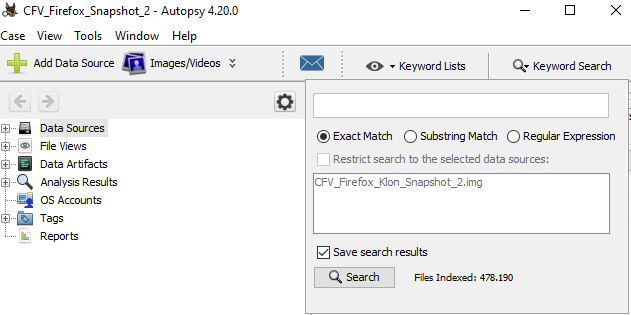
\includegraphics{bilder/autopsy-search.png}}
%	\label{...}
	\caption{Tabelle mit wiederherstellbaren Dateien: Logfile 1 vs. Logfile 2}
\end{figure}

Zusätzlich kategorisiert Autopsy beim Einlesen eines Festplatten-Images automatisch die Dateien. Für jede Kategorie werden die kategorisierten Dateien nach PB Artefakten untersucht. Für diesen Versuch sind folgende Dateikategorien von Interesse:
\begin{itemize}
\item Web Bookmarks
\item Web Cookies
\item Web History
\item Web Categories
\end{itemize}

Sowohl die Stichwortsuche als auch die Analyse der kategorisierten Dateien wird für jedes Festplatten-Image durchgeführt.

\subsubsection*{Analyse mit Volatility}

Bei der Analyse des Arbeitsspeichers als Uncommon Location ist es kritisch, dass ein gefundener String eindeutig einem Browserprozess zugeordnet werden kann. 

In der Literatur wird der Arbeitsspeicher oft analysiert, indem der vollständige RAM-Dump als Binärdatei in einem Hexadezimaleditor wie HxD geöffnet wird, um danach eine Stringsuche durchzuführen. \cite{Rochmadi.2017, Md.2018, Montasari.2015}
Ein in der Binärdatei gefundener String ist jedoch kein Indiz, dass das Artefakt tatsächlich im Zusammenhang mit dem Browsing Szenario steht.
Wie in Abbildung X und Y gezeigt, wird ein String, der in einer Textdatei auf dem Desktop gespeichert ist ebenfalls im Hexadezimaleditor HxD angezeigt, obwohl kein Browsing Szenario durchgeführt wurde.
\begin{figure}[h!]
	\resizebox{0.5\linewidth}{!}{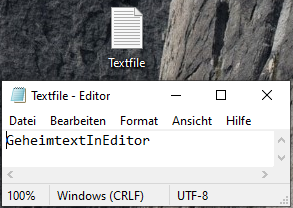
\includegraphics{bilder/ram-editor1.png}}
%	\label{...}
	\caption{Tabelle mit wiederherstellbaren Dateien: Logfile 1 vs. Logfile 2}
\end{figure}
\begin{figure}[h!]
	\resizebox{\linewidth}{!}{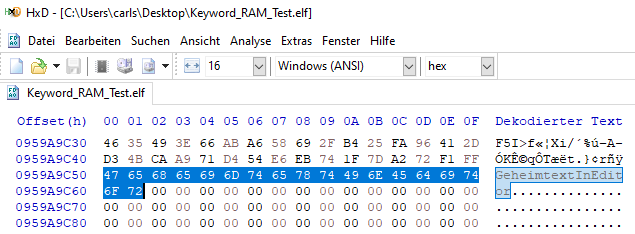
\includegraphics{bilder/ram-editor2.png}}
%	\label{...}
	\caption{Tabelle mit wiederherstellbaren Dateien: Logfile 1 vs. Logfile 2}
\end{figure}

Aus diesem Grund wird das forensische Tool "Volatility" zur Analyse des Arbeitsspeichers verwendet. 
Bei den Common Locations wurde Volatility ausschließlich zur Dateiextraktion genutzt.
Um einen im RAM gefundenen String einem Browserprozess zuordnen zu können, wird das Volatility PlugIn "Yarascan" verwendet.

YARA ist eine flexibles regelbasiertes Tool, das verwendet werden kann, um nach bestimmten Mustern, Signaturen oder Verhaltensmerkmalen im Arbeitsspeicher zu suchen. Dazu werden sogenannte "YARA-Regeln" verwendet. Dabei handelt es sich um eine domänenspezifische Skriptsprache, mithilfe dieser zu suchende Strings und Muster definiert werden.
Die für diesen Versuch verwendeten Yara-Regeln sind einfache String-Pattern, die jeden Schritt des Browsing-Szenarios abdecken. 
Neben den in Tabelle X in Kapitel X definierten Strings der PB Artefakte, wurde eine zusätzliche "HTML-Regel" eingeführt \cite{Said.2011}. Diese Regel sucht nach HTML-Fragmenten, die eindeutig zu einer besuchten Seite des Browsing-Szenarios zuzuordnen sind
Die für diesen versuch verwendeten Yara-Regeln sind im Anhang X (TODO!) gezeigt.
Um den RAM-Dump nach den Yara-Regeln zu durchsuchen wird folgender Befehl ausgeführt: \texttt{vol.py -f ram\_dump.img windows.vadyarascan --yara-file yara\_rules.yara > yarascan.txt}
Nachdem der RAM-Dump nach den Regeln durchsucht wurde, liefert Yarascan eine Ausgabe mit allen gefundenen Strings.
%	*** TODO: Erklärung Yara-Ausgaben, mit Screenshot ***
Für jeden Treffer liefert Yarascan die PID des Prozesses, in dem der String gefunden wurde sowie virtuelle Adresse des gefundenen Strings.

\begin{figure}[h!]
	\centering
	\small
	\centerline{\resizebox{\linewidth}{!}{\input{bilder/yarascan_plugin_tree-Latex.pdf_tex}}}
	\caption{TODO: Process Monitor Write Operation to Excel Spreadsheet}
	\label{fig:jes}
\end{figure}
Wie in Abbildung X dargestellt, bildet Yarascan die Grundlage der RAM-Analyse.
Davon ausgehend weden mit dem Plugin "pslist" der Prozessname zur PID des Prozesses ermittelt, in dem der String gefunden wurde. Dazu wird folgender Befehl ausgeführt: \texttt{vol.py -f ram\_dump.img windows.pslist > pslist.txt}

Oft ist für bei einem gefundenen String von Interesse, ob in den Speicheradressen vor und nach dem Treffer weitere Zusammenhänge erkennbar sind.
Dazu wird mithilfe des Plugins "memmap" zunächst die Abbildung der virtuellen Speicheradressen eines Prozesses auf den Byte-Offset in der Speicherseite des Prozesses:
\texttt{vol.py -f ram\_dump.img windows.memmap --pid <PID> > memmap.txt}
Diese Seite kann mithilfe des "--dump" Flags extrahiert werden: \texttt{vol.py -f ram\_dump.img -o \\dump\_dir\\ windows.memmap --pid <PID> --dump}
Wenn die extrahierte Seite mit einem Hexadezimaleditor wie HxD geöffnet wird, kann der String-Treffer anhand des ermittelten Byte-Offsets gefunden werden.


\subsection{Registry}

Die letzte Kategorie analysierter Daten umfasst die Artefakte der Registry.
Diese zählen sowohl zu den Common als auch Uncommon Locations und werden deshalb eigene Kategorie aufgeführt.

\paragraph*{Common Locations}

*** TODO: Common location: Shellactivities Key ***
	existiert nicht mehr --> Nicht mehr vorhanden in aktueller Version (Verweis auf E-Mail)

Als Teil der Common Locations werden die Registry-Aktivitäten in den Process Monitor Logfiles analysiert.
Dazu wird jede Logfile in Process Monitor eingelesen und wie in Abbildung X gezeigt gefiltert.
\begin{figure}[h!]
	\resizebox{\linewidth}{!}{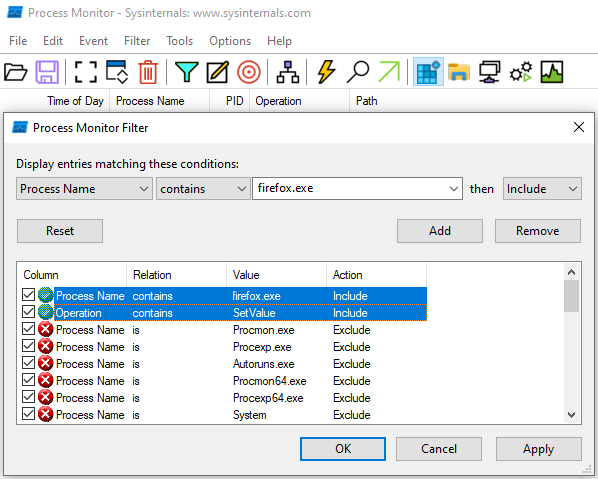
\includegraphics{bilder/process-monitor-filter-registry.png}}
%	\label{...}
	\caption{Tabelle mit wiederherstellbaren Dateien: Logfile 1 vs. Logfile 2}
\end{figure}
Zunächst wird ausschließlich die Option "Registry Activity" ausgewählt.
Anschließend wird nach Browser-Prozessnamen analog zu den Schreiboperationen in Kapitel X gefiltert.
Das gefilterte Logfile wird als CSV Datei exportiert und in Excel weiter verarbeitet.
Zunächst werden gleiche Schreiboperationen gelöscht.
Anschließend werden die geschriebenen Registry Keys browserspezifisch gruppiert.
	
\paragraph*{Uncommon Locations}
Als Uncommon Location werden alle Registry Hives in jedem Festplatten-Image mit dem "Registry Explorer" untersucht.
Jedes Hive hat eine bestimmte Funktion, wie die Speicherung von Systemeinstellungen (System-Hives) oder individuellen Benutzerkonfigurationen (User-Hives). Diese in Tabelle X dargestellten Hives werden von Windows beim Start geladen und dienen als Quelle für Einstellungen und Informationen, die von verschiedenen Systemkomponenten und Anwendungen genutzt werden.	
 % https://medium.com/@haircutfish/tryhackme-windows-forensics-1-task-3-accessing-registry-hives-offline-task-4-data-acquisition-b440f5be2a13
Zur Analyse wird jeder Hive aus einem VM-Snapshot extrahiert und in eine Registry Explorer Sitzung geladen, anschließend wird eine Stringsuche nach PB Artefakten in allen geladenen Hives gleichzeitig durchgeführt.

\begin{table}[h!]
%\resizebox{\linewidth}{!}{
\begin{tabular}{lllll}
\cline{1-2}
\multicolumn{2}{|c|}{\textbf{System-Hives (C:\textbackslash{}\textbackslash{}Windows\textbackslash{}\textbackslash{}System32\textbackslash{}\textbackslash{}Config)}} &  &  &  \\ \cline{1-2}
\multicolumn{1}{|l|}{\textbf{Dateiname}}             & \multicolumn{1}{l|}{\textbf{Inhalt}}                                                                           &  &  &  \\ \cline{1-2}
\multicolumn{1}{|l|}{\textit{DEFAULT}}               & \multicolumn{1}{l|}{Standardkonfigurationseinstellungen für neue Benutzerprofile.}                             &  &  &  \\ \cline{1-2}
\multicolumn{1}{|l|}{\textit{SAM}}                   & \multicolumn{1}{l|}{Sicherheitskontensdaten, einschließlich der Benutzerkonten und deren Kennwörter.}          &  &  &  \\ \cline{1-2}
\multicolumn{1}{|l|}{\textit{SECURITY}}              & \multicolumn{1}{l|}{Sicherheitsinformationen für die Zugriffssteuerung und Authentifizierung.}                 &  &  &  \\ \cline{1-2}
\multicolumn{1}{|l|}{\textit{SOFTWARE}}              & \multicolumn{1}{l|}{Konfigurationsdaten für installierte Software und Anwendungen.}                            &  &  &  \\ \cline{1-2}
\multicolumn{1}{|l|}{\textit{SYSTEM}}                & \multicolumn{1}{l|}{Systemkonfigurationseinstellungen und Gerätetreiberinformationen.}                         &  &  &  \\ \cline{1-2}
                                                     &                                                                                                                &  &  &  \\ \cline{1-2}
\multicolumn{2}{|c|}{\textbf{User-Hives (C:\textbackslash{}\textbackslash{}Users\textbackslash{}\textbackslash{}\textless{}username\textgreater{})}}                  &  &  &  \\ \cline{1-2}
\multicolumn{1}{|l|}{\textbf{Dateiname}}             & \multicolumn{1}{l|}{\textbf{Inhalt}}                                                                           &  &  &  \\ \cline{1-2}
\multicolumn{1}{|l|}{\textit{NTUSER.DAT}}            & \multicolumn{1}{l|}{Individuelle Einstellungen und Konfigurationen für den angemeldeten Benutzer}              &  &  &  \\ \cline{1-2}
\multicolumn{1}{|l|}{\textit{USRCLASS.DAT}}          & \multicolumn{1}{l|}{Dateizuordnungen und Registrierungseinstellungen für den angemeldeten Benutzer}            &  &  &  \\ \cline{1-2}
\end{tabular}
%}
\end{table}
	

